%
% File: chap01.tex
% Author: Liam O'Shea
% Description: Introduction chapter where the boxing goes.
%
\let\textcircled=\pgftextcircled
\chapter{Implementation}
\label{chap:intro}

\initial{B}egging implementation chapter. How the hell do I start this. What even goes here.

%=======
\section{Comparison Methods}
\label{sec:sec01}


I began by plotting the initial Kinect Data over time in an attempt to understand \& visualise the nature of the data. I differentiated the data as a method of smoothing and to get the velocity data from distance.


\begin{figure}[t!]
\centering
\begin{minipage}{6.0cm}
    \centering
    \subtop[]{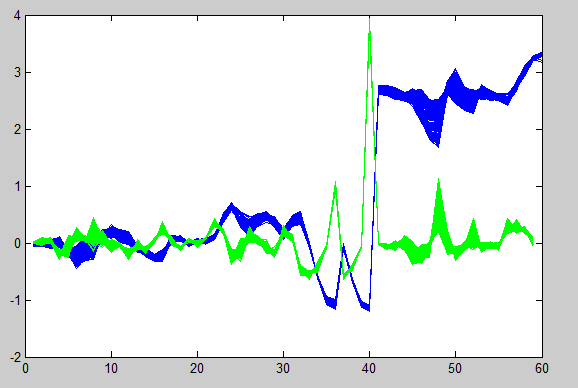
\includegraphics[height=0.25\textheight]{fig04/fig06}}
    \label{fig:1}
\end{minipage}
\begin{minipage}{6.0cm}
    \centering
    \subtop[]{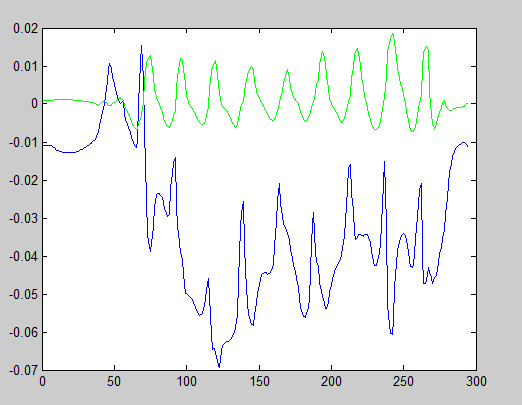
\includegraphics[height=0.25\textheight]{fig04/fig07}}
    \label{fig:2}
\end{minipage}
\mycaption[ALLData] {(a) Kinect Skeleton vs Time. 
(b) Hip Joint vs Time, Blue = Raw data, Green = Differentiated data.}
\end{figure}

After recording a punch sequence my first inclination was to look at the left hand (jab) over time. I plotted the z co-ordinate of the left wrist joint over each frame which produced a periodic pattern for which looked promising.


\begin{figure}[h]
    \centering
    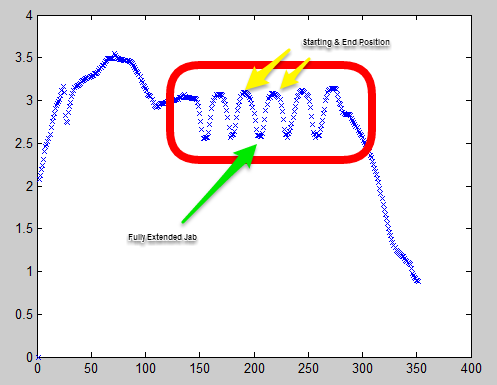
\includegraphics[height=0.25\textheight]{fig04/fig01}
    \mycaption[Kinect Device]{Depth of left wrist joint over time}
    \label{fig:kinect}
\end{figure}



My next step was to look at  punch segmentation. Due the cyclical nature of the punch movement I needed to develop a method for segmenting the punches. I decided the best way to do this was to smooth the signal and use local maxima/minima as a means of successfully segmenting the beginning and end of each punch. As you can see from Figure 4.2 some smoothing was required due to local maxima/minima which did not signify the beginning or end of a punch.



\begin{figure}[h]
\centering
\begin{minipage}{6.0cm}
    \centering
    \subtop[]{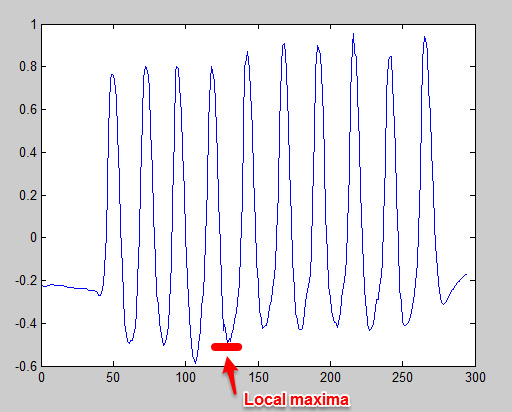
\includegraphics[height=0.25\textheight]{fig04/fig02}}
    \label{fig:kinect}
\end{minipage}

\hspace{0.5cm}
\begin{minipage}{6.0cm}
    \centering
    \subtop[]{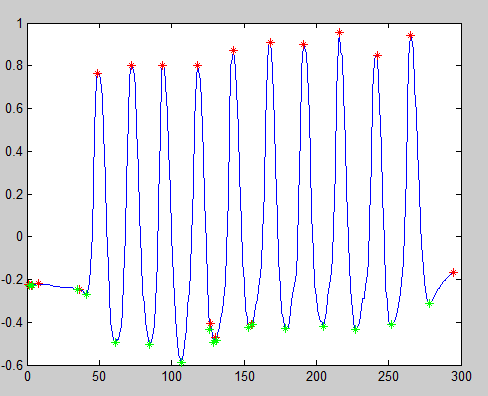
\includegraphics[height=0.25\textheight]{fig04/fig04}}
    \label{fig:kinect2}
\end{minipage}
\begin{minipage}{3.5cm}
    \centering
    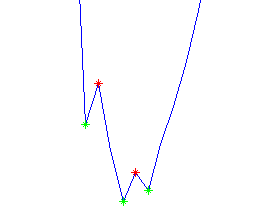
\includegraphics[height=0.15\textheight]{fig04/fig05}
    \label{fig:kinect3}
\end{minipage}
\mycaption[WAT]{(a) Periodic punch signal over time (frame number).(b) Periodic signal with local maxima/minima labelled. (c) Close up of local maxima/minima.}
\end{figure}


Smoothing.
I looked at using differentiation as a means of obtaining the velocity and using that as a sensible measure to mark my punches. This did a good job of smoothing out the curve which would allow me to successfully segment my punches. 


\begin{figure}[h]
    \centering
    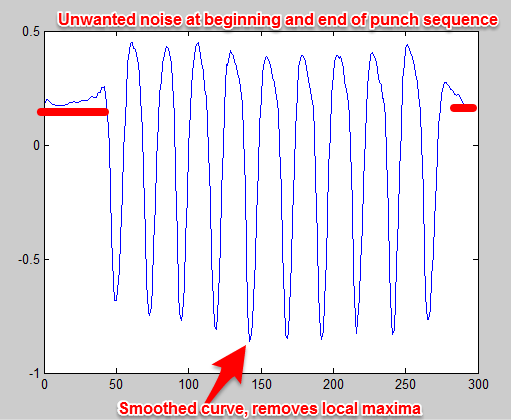
\includegraphics[height=0.25\textheight]{fig04/fig03}
    \mycaption[Kinect Device]{Depth of left wrist joint over time}
    \label{fig:kinect}
\end{figure}


\paragraph {Dimensionality Reduction Comparison}
It was important to find a way to successfully reduce my data into a cyclical signal that I could automatically segment. I tested a variety of both linear and non-linear techniques (see design section) and analysed the principal components produced. Despite PCA being an older, simple technique than more modern techniques such as diffusion maps it actually produced the most uniform, cyclical signal for the first component making it an obvious choice.

{\bf Maybe talk about using LTSA here in some way as a second component}




\begin{figure}[h]
\centering
\begin{minipage}{6.0cm}
    \centering
    \subtop[]{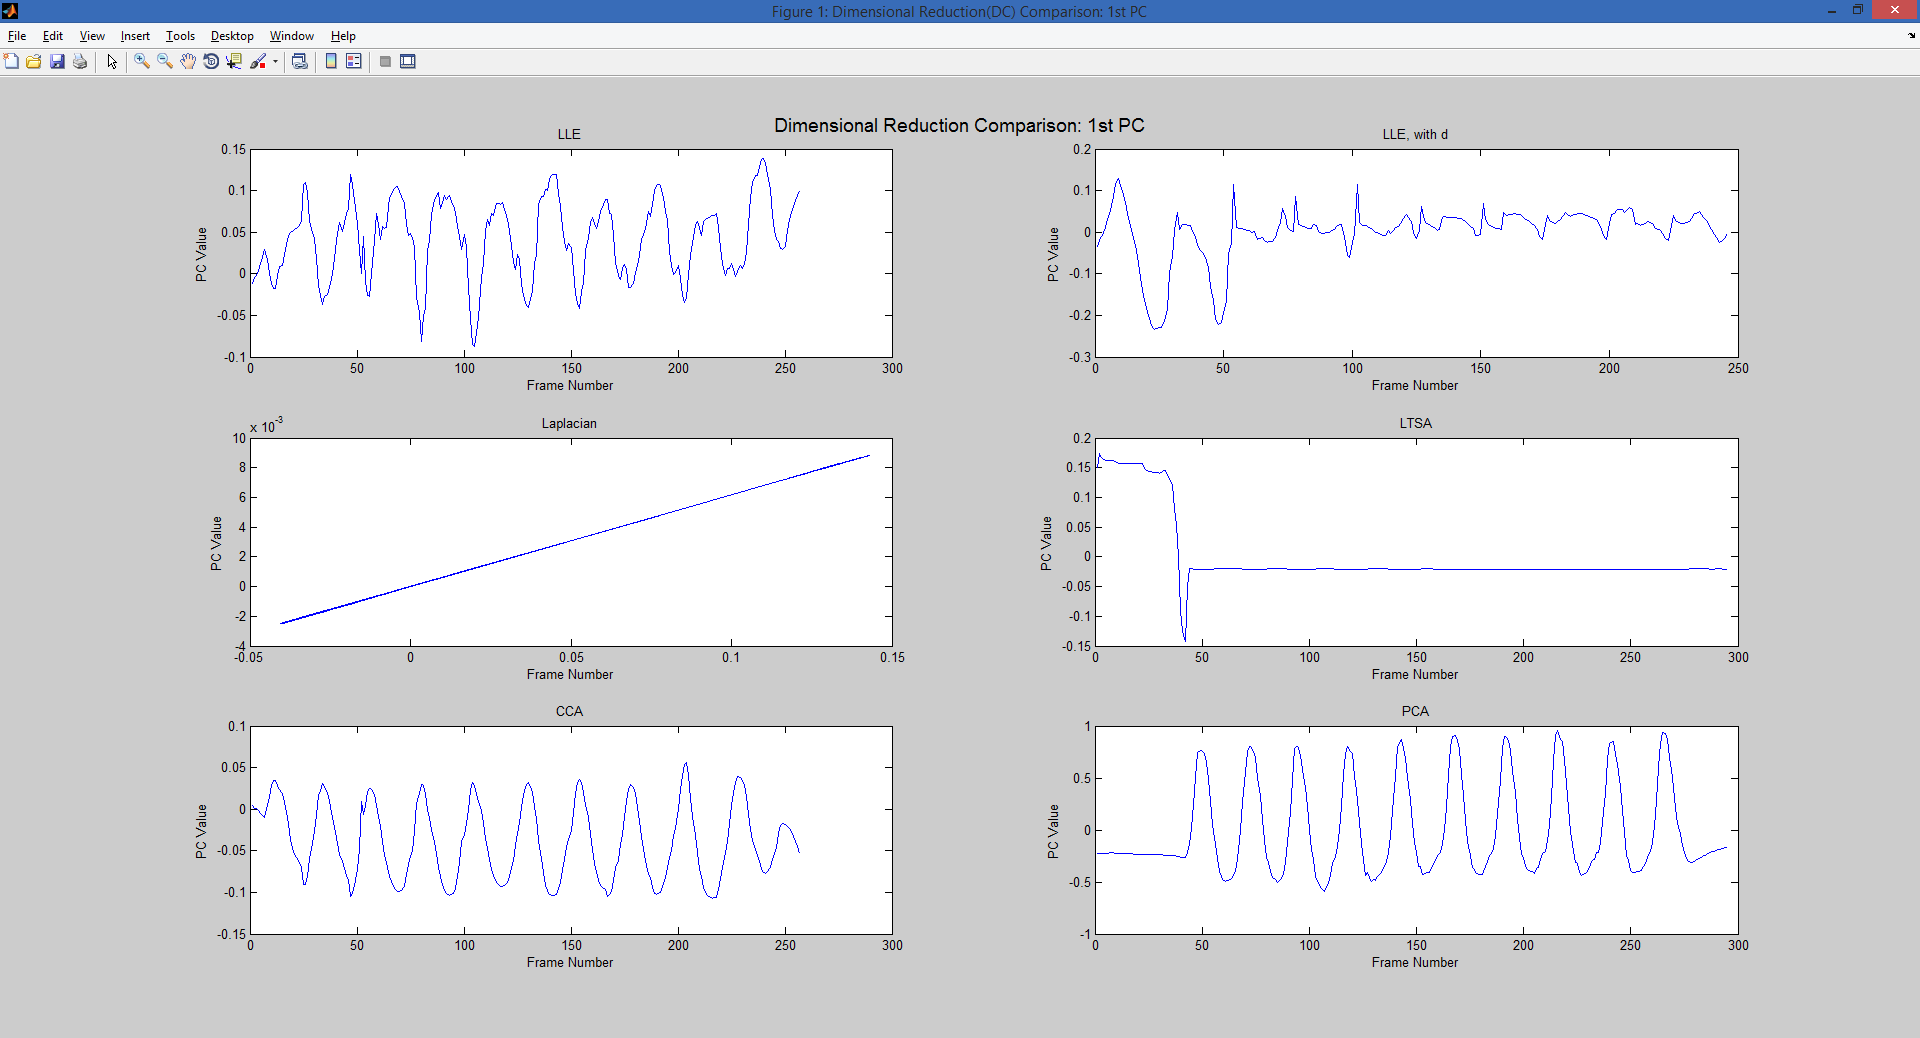
\includegraphics[height=0.25\textheight]{fig04/fig08}}
    \label{fig:kinect}
\end{minipage}
\hspace{0.5cm}
\begin{minipage}{6.0cm}
    \centering
    \subtop[]{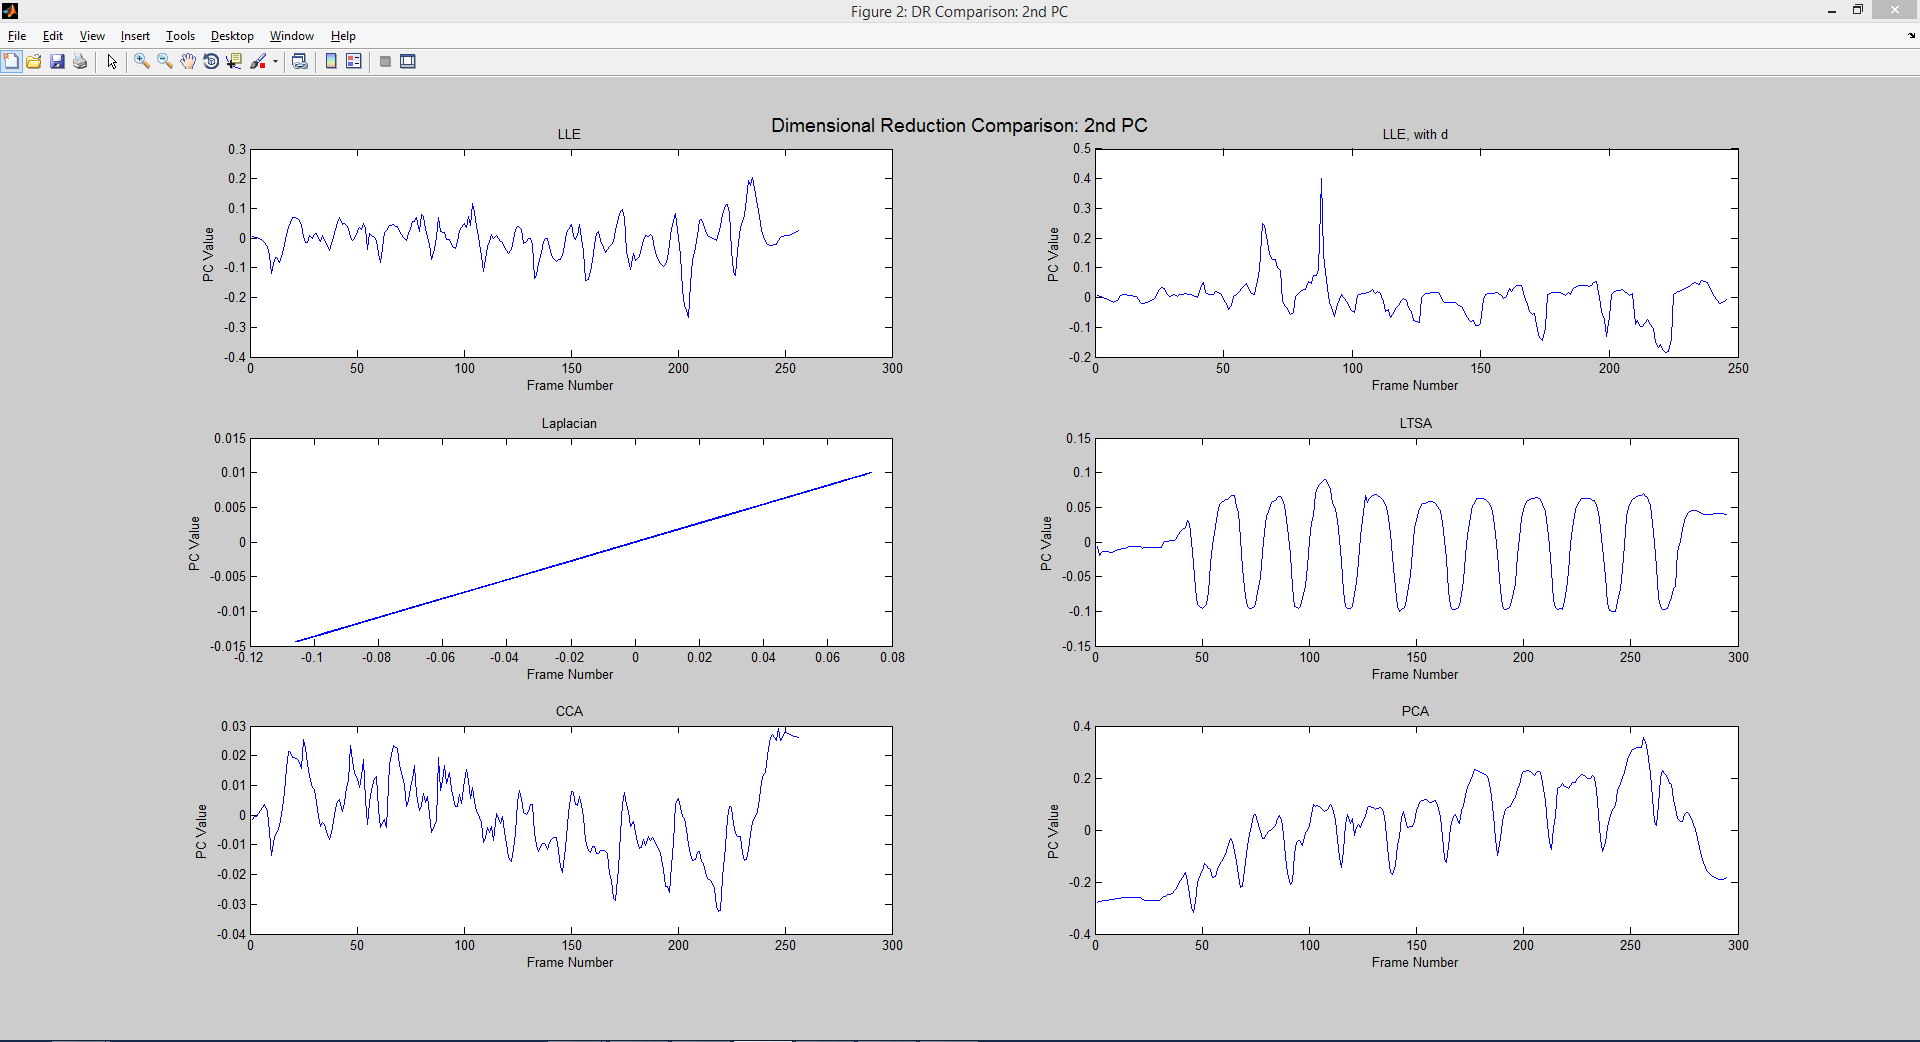
\includegraphics[height=0.25\textheight]{fig04/fig09}}
    \label{fig:kinect2}
\end{minipage}
\begin{minipage}{6.0cm}
    \centering
    \subtop[]{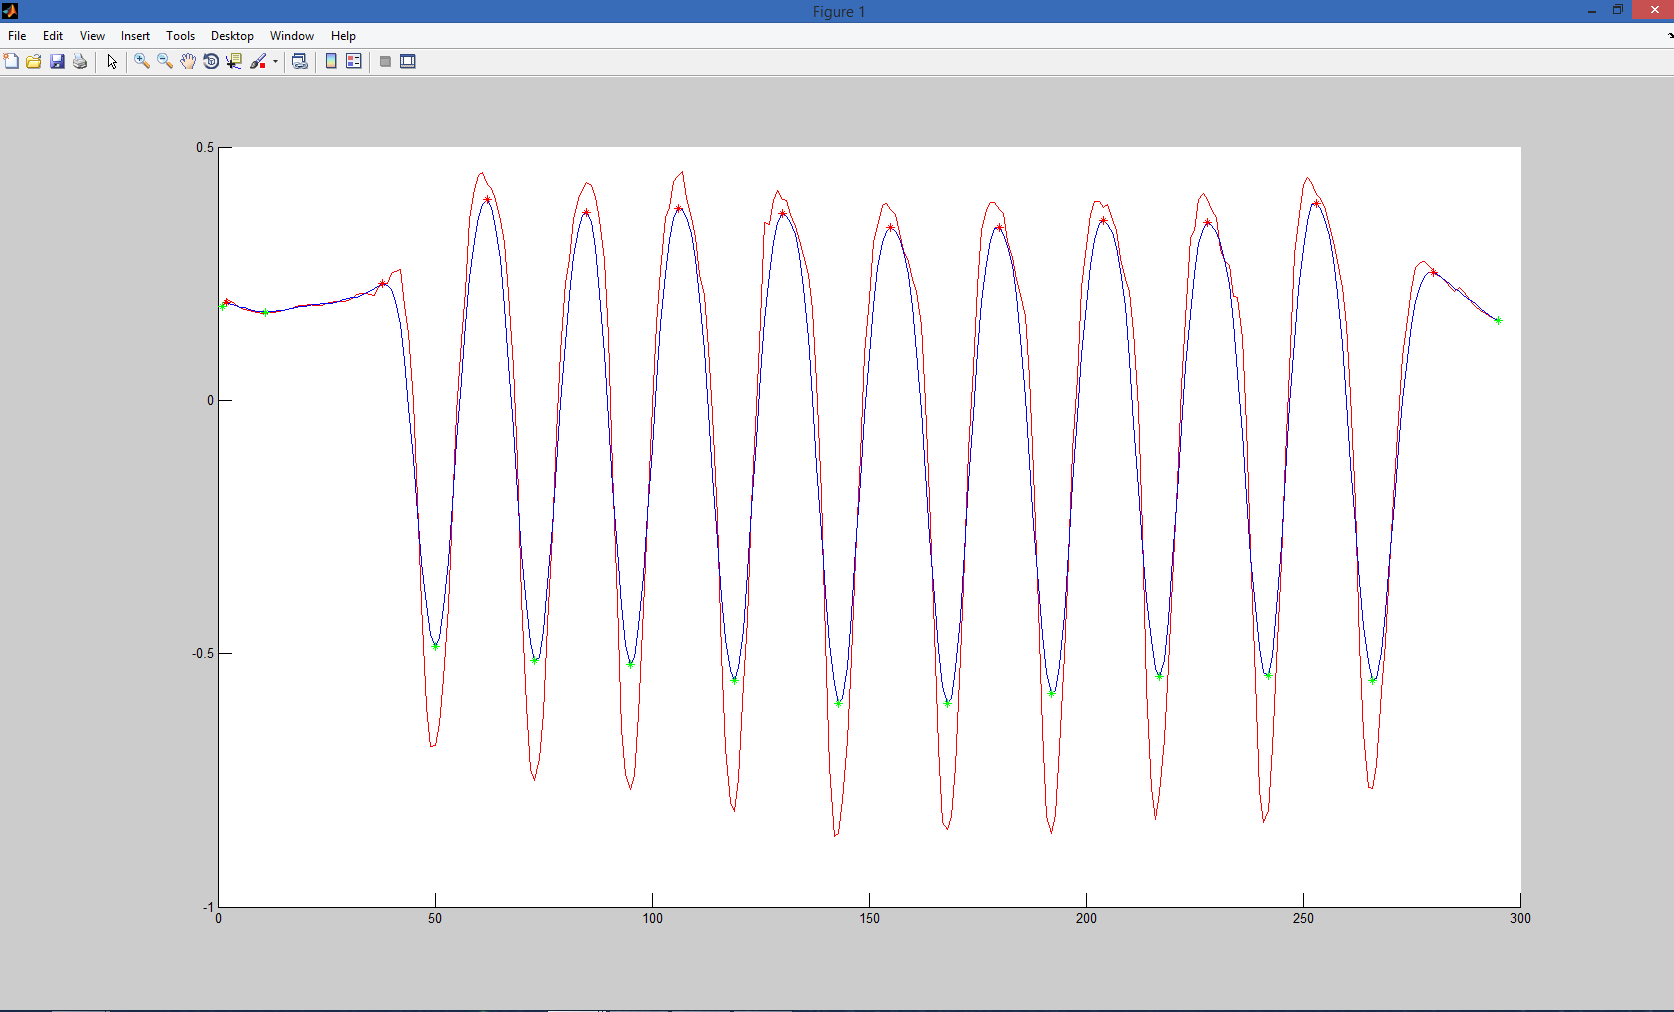
\includegraphics[height=0.25\textheight]{fig04/fig10}}
    \label{fig:kinect2}
\end{minipage}
\mycaption[WAT]{(a) Comparison of Dimensionality Reduction Techniques. PLotting first and second principal components.}
\end{figure}



Now lets see the first Principal Component (from PCA) for each punch.
TALK about normalisation of data.
Talk about getting better data.

\begin{figure}[h]
    \centering
    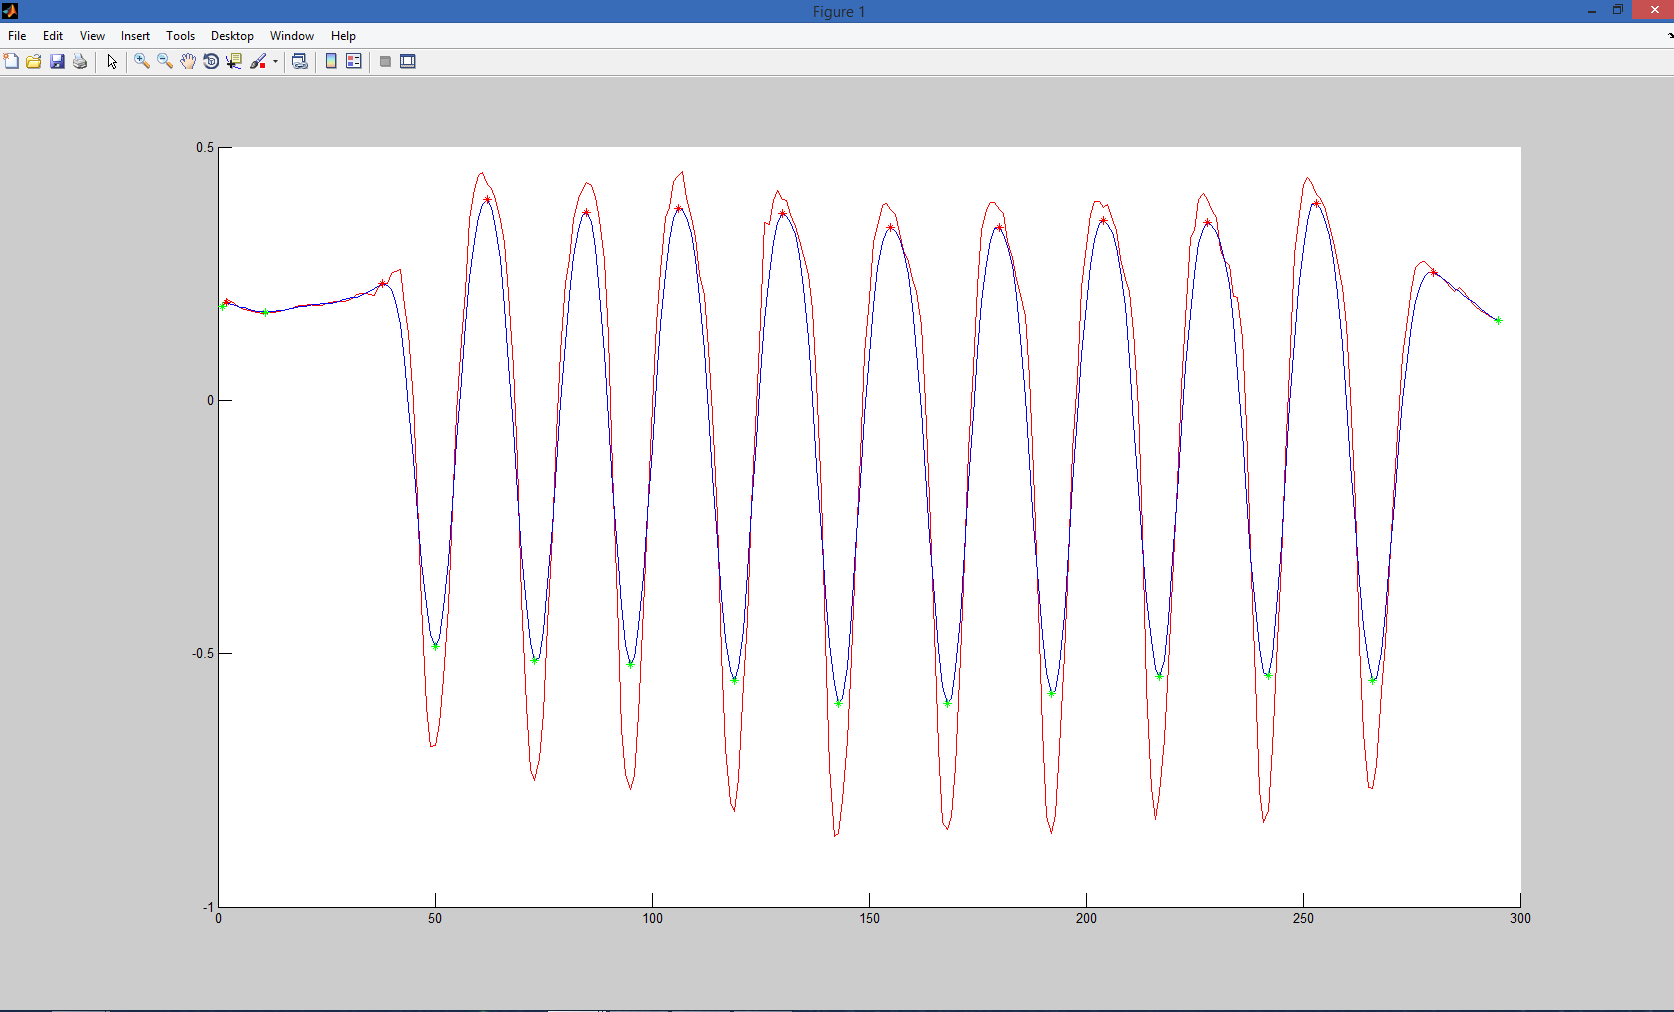
\includegraphics[height=0.25\textheight]{fig04/fig10}
    \mycaption[Kinect Device]{Depth of left wrist joint over time}
    \label{fig:kinect}
\end{figure}


\paragraph{Automated Punch Segmentation}
After obtaining a smooth cyclical representation of the Jab



\paragraph{Heuristic Rules}



{\bf Hidden Markov models?}
Chapter 4: Implementation\newline
Chapter 5: Data capture??\newline
Need to make and collect data consent forms to run a study?\newline
Need to gather more data?\newline

\paragraph{Data Format}
I record data from the Kinect in a space separated text file with each line corresponding to one timeframe. The structure of a line is: 
tracking_flag x_0 y_0 z_0 tracking_flag x_1 y_1 z_1 ... tracking_flag x_19 y_19 z_19,
where x_i,y_i,z_i are the x,y,z coordinates representing the position of the ith joint.
Each new line is represented by a very large value that could not represent a Kinect measurement. (e.g. 2000000) 
The tracking_flag is an integer which describes the status of the joint:
Joint not tracked = 0, Joint position inferred = 1, Join position tracked = 2.
If the joint is not tracked the position is set to (-10000, -10000, -10000) and it should not be used.
The position of the camera is (0,0,0).


\begin{center}
    \begin{tabular}{| l | l |}
    \hline
    Joint Number & Joint Name \\ \hline
    0 & NUI_SKELETON_POSITION_HIP_CENTER \\ \hline
    1 & NUI_SKELETON_POSITION_SPINE\\ \hline
    2 & NUI_SKELETON_POSITION_SHOULDER_CENTER\\ \hline
    3 & NUI_SKELETON_POSITION_HEAD\\ \hline
    4 & NUI_SKELETON_POSITION_SHOULDER_LEFT\\ \hline
    5 & NUI_SKELETON_POSITION_ELBOW_LEFT\\ \hline
    6 & NUI_SKELETON_POSITION_WRIST_LEFT\\ \hline
    7 & NUI_SKELETON_POSITION_HAND_LEFT\\ \hline
    8 & NUI_SKELETON_POSITION_SHOULDER_RIGHT\\ \hline
    9 & NUI_SKELETON_POSITION_ELBOW_RIGHT\\ \hline
    10 & NUI_SKELETON_POSITION_WRIST_RIGHT\\ \hline
    11 & NUI_SKELETON_POSITION_HAND_RIGHT\\ \hline
    12 & NUI_SKELETON_POSITION_HIP_LEFT\\ \hline
    13 & NUI_SKELETON_POSITION_KNEE_LEFT\\ \hline
    14 & NUI_SKELETON_POSITION_ANKLE_LEFT\\ \hline
    15 & NUI_SKELETON_POSITION_FOOT_LEFT\\ \hline
    16 & NUI_SKELETON_POSITION_HIP_RIGHT\\ \hline
    17 & NUI_SKELETON_POSITION_KNEE_RIGHT\\ \hline
    18 & NUI_SKELETON_POSITION_ANKLE_RIGHT\\ \hline
    19 & NUI_SKELETON_POSITION_FOOT_RIGHT\\ \hline
    \hline
    \end{tabular}
\end{center}
%=========================================================